\documentclass[12pt, a4paper]{article}
\usepackage[utf8]{inputenc}
\usepackage[IL2]{fontenc}
\usepackage[czech]{babel}
\usepackage{graphicx}
\usepackage{verbatimbox}
\usepackage{float}

\begin{document}
\begin{figure}[h!]
\centering

\includegraphics[bb= 0 0 820 445 , width=75mm]{favlogo.jpg}
\end{figure}

\vspace{5cm}

{\centering
{\huge Hra Milostný Dopis}\\[1em]
{\large KIV/UPS - 1. semestrální práce}\\[7,5cm]
}

\begin{tabular}{l r}
student: & Radek VAIS\\
os. číslo: & A13B0457P\\
mail: & vaisr@students.zcu.cz\\
datum: & 10.1.2017\\
\end{tabular}

\thispagestyle{empty}
\newpage

%========================================
%========================================
%========================================
%========================================
%========================================
\section{Zadání} %=====================================================================================================

Vypracujte dva programy (klient a server) pro počítačovou simulaci karetní hry Milostný dopis. Navrhněte vlastní komunikační protokol, který bude využívat transportní protokol TCP nebo UDP k doručování zpráv.

Server bude akceptovat parametry pro základní nastavení (port, adresu pro naslouchání). Bude zpracován v programovacím jazyce C/C++ a cílová platforma bude Linux. Pro práci se sítí bude využívat implementaci BSD soketů.

Klient bude zpracován v programovacím jazyce Java. Nutnou součástí klienta je alespoň minimální uživatelské rozhraní. Klient musí být kompatibilní s operačními systémy Windows i Linux.  

Hotovou práci odevzdejte po osobním předvedení v laboratoři KIV UC326 na Portál.

%========================================
%========================================
%========================================
%========================================
%========================================
\newpage
\section{Analýza~úlohy} %============================================================================================

\subsection{Pravidla hry}

Milostný dopis je karetní hra pro až čtyři hráče. Hráči se symbolicky snaží doručit dopis princezně a získat tak její přízeň. Každý hráč má v ruce jednu kartu s postavou, která symbolizuje kdo právě nese milostný dopis pro princeznu. Hráč co je na tahu si dobere druhou a s této dvojice vybere kartu jejíž efekt se uskuteční. Po uskutečnění efektu kartu vyloží před sebe a pokračuje další hráč, který zatím nebyl eliminován. 

\begin{figure}[ht]
\centering
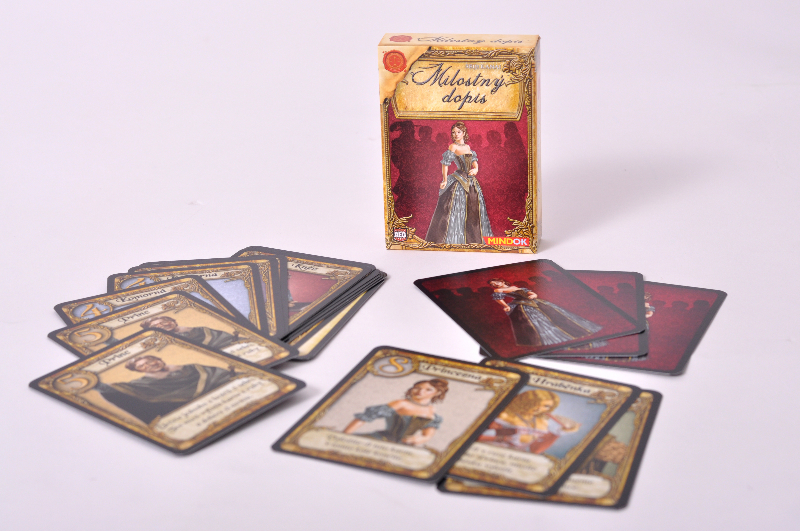
\includegraphics[bb= 0 0 800 531 , height=5cm]{hra_fyz.jpg}
\caption{Ukázka fyzické hry.}
\label{fig:game}
\end{figure}

Konec hry nastává ve chvíli, kdy dojdou karty v balíčku nových karet nebo zbývá ve hře poslední hráč. Vítězem kola je hráč, který nebyl v kole eliminován a drží nejvyšší kartu. Složení karet v balíčku viz Tabulka \ref{tab:karty}. Celé znění pravidel naleznete v přiloženém souboru pravidla.pdf.

\begin{table}[ht]
\centering
\begin{tabular}{|c | p{7cm} | c|}
\hline
Název karty (hodnota) &  Stručný efekt & Počet v balíčku\\
\hline
Strážná (1) & Eliminuje protihráče & 5\\
\hline
Kněz (2) & Zjistí kartu protihráče & 2\\
\hline
Baron (3) & Eliminuje hráče s nižší kartou & 2 \\
\hline
Komorná (4) & Ochrání před efekty karet & 2 \\
\hline
Princ (5) & Přinutí vyložit kartu & 2\\
\hline
Král (6) & Vyměním si kartu s protihráčem & 1\\
\hline
Hraběnka (7)& Musí být vyložena při kombinaci s Princem nebo králem & 1\\
\hline
Princezna (8)& Při jejím odhalení jsem eliminován & 1\\
\hline
\end{tabular}
\label{tab:karty}
\caption{Stručný popis karet v balíčku.}
\end{table}


\subsection{Zpracování požadavků na serveru}

Zásadním problémem při návrhu serveru je způsob zpracování požadavků. Je třeba zajistit paralelizaci požadavků aby nedocházelo k blokování serveru náročnými operacemi. Problém je vhodně zvolit rozložení požadavků mezi pracující vlákna. Existuje několik přístupů: každý klient jedno vlákno, každý požadavek jedno vlákno, každá hra jedno vlákno, \ldots Z této množiny jsem vybral několik variant.

\subsubsection{Každý požadavek jedno vlákno}
V této variantě se při přijetí požadavku vytvoří vlákno, které zpracuje požadavek (zprávu) a poté ukončí svůj životní cyklus. Uvažujeme li tento návrh je program zbytečně zatěžován vytvářením a ukončováním nových vláken. Nelze predikovat počet souběžných požadavků (každý klient může v jeden okamžik vyžadovat více informací), proto je možné, že se velice snadno program dostane na limitní počet vláken. V případě jednoduchých požadavků typu \emph{getHodnota} je vysoce neefektivní vytvářet nové vlákno. Výhodou této varianty je paralelní provádění všech požadavků.

\subsubsection{Každý klient/hra jedno vlákno}

V této variantě s každým vytvořeným klientem vytvoříme vlákno, které zpracovává požadavky klienta. Tato varianta se zdá přijatelnější. V případě náročného požadavku klient blokuje pouze sám sebe a nezdržuje ostatní hráče. Opět nelze předem predikovat počet klientů. Další nevýhodou je sekvenční zpracování požadavků klienta.

Můžeme počet vláken snížit změnou metodiky na vytváření vláken pro jednotlivé hry. Zde vyvstává problém, kdy dojde k vytvoření vlákna hry. Potřebujeme tedy další jedno netriviální vlákno programu, které obstarává prvotní připojení klientů a požadavky na vytvoření a zařazení do her. Za předpokladu, že počet vláken hráčů je $N$ potom je zlepšení využití vláken minimálně $N/2 + 1$ v případě her více hráčů ještě lepší.

\subsubsection{Několik vláken zpracovává zprávy}

Jako nejvhodnější varianta se jeví kombinace obou předchozích metod. Z druhé metody jako přednost volím jedno specializované vlákno. V tomto případě jedno specializované vlákno pouze na příjem zpráv. Po přijetí bude zpráva zařazena do fronty k dalšímu zpracování. Pro zpracování takto získaných zpráv použijeme předem stanovený počet pracujících vláken. Požadavky jsou zpracovávány dle návrhového vzoru Producent - Konzument, kde producent je vlákno zpracovávající příchozí zprávy a konzumentem jsou pracující vlákna. Zde je zachován paralelní běh různých operací a zároveň máme předem jasně stanovený počet vláken, který lze nastavit dle zatížení serveru.

\subsection{Protokol}
V případě použití protokolu UDP, je třeba v uživatelském protokolu definovat opravné vlastnosti, pro případ "zatoulání" zprávy na síti. Dále je třeba v hlavičce každé zprávy definovat příjemce a odesílatele. V případě TCP je třeba pouze autentizovat uživatele na soketu a předpokládat možnost spojení více aplikačních zpráv do jedné zprávy.

Pro tento školní případ je z důvodů nižších nároků na vlastnosti uživatelského protokolu akceptovatelné použít protokol TCP. 

%========================================
%========================================
%========================================
%========================================
%========================================
\section{Popis~implementace} %=======================================================================================


\subsection{Komunikační protokol}

Pro jasné označení začátku zprávy je použitá sekvence tří znaků \texttt{\#} následují právě čtyři místa pro číslice, které označují celkovou délku zprávy. Za délkou zprávy následují dva tříznakové kódy, které určují kategorii zprávy. Tuto hlavičku uzavírá jeden znak \texttt{\#}. Bezprostředně za hlavičkou následuje tělo zprávy. Zpráva může vypadat například takto:

\begin{verbatim}
                ###0019LOGECH#Honza
\end{verbatim}

Tímto typem zprávy se uživatel registruje na serveru. Všechny možné typy zpráv jsou uvedeny v následujících tabulkách (Tabulky 2 - 5). Server vždy validuje práva na provedení operace definované ve zprávě. Může odpovědět negativně (v případě přihlašování musí), ale také může zaslanou zprávu, ke které není oprávnění ignorovat.

\begin{table}[H]%=======================================================================================
\centering
Datové typy ve zprávě
\begin{tabular}{| p{3cm} | p{10cm} |}
\hline
Datový typ &  popis\\
\hline
karta & číslo 1 - 9 \\
\hline
ID hráč & pět alfanumerických znaků\\
\hline
ID hra & GAMExx - kde xx jsou libovolná písmena \\
\hline
počet kol & libovolné číslo \texttt{uint}  \\
\hline
počet hráčů & 2 - 4 \\
\hline
záznam hry & [ID hry]    \&\&    [počet hráčů (přihlášených)]    \&\&    [odstartovaná] \\
\hline
status hráče & [ID hráče]    \&\&    [alive]    \&\&   [token]    \&\&    [guarded]  \\
\hline
výsledek karty & OK nebo CANCEL \&\& WRONG/MISS/GUARDED - dle typu výsledku\\
\hline
\end{tabular}
\label{tab:zpravyDatTypy}
\caption{Možné datové struktury použité ve zprávě}
\end{table}


\begin{table}[H]%=======================================================================================
\centering
Primární kód LOG (login, přihlašvání)
\begin{tabular}{|c | c | p{4cm} | p{5cm} |}
\hline
Druhý kód &  Zdroj & Obsah zprávy & Smysl zprávy\\
\hline
ECH & Klient & [Přezdívka uživatele] & Registrace na serveru \\
\hline
COD & K &[ID hráče] & Opětovné přihlášení\\
\hline
OUT & K &[ID hráče] & Odhlášení ze serveru \\
\hline
ACK & Server &[ID hráče]    \&\&    [Přezdívka] & Potvrzení přihlášení / registrace \\
\hline
NAK & S &[ID hráče]    \&\&    [Přezdívka] & Odmítnutí duplicitního přihlášení klienta na jednom serveru \\
\hline
NAK & S &NO ID & Odmítnutí přihlášení klienta (neznámé id, nedostatek zdrojů) \\
\hline
\end{tabular}
\label{tab:zpravyLOGServer}
\caption{Možné typy zpráv dle kategorie login. Tato kategorie slouží pro registraci a přihlašování uživatele k serveru}
\end{table}

\begin{table}[H]%=======================================================================================
\centering
Primární kód GAM (game, hra) - zdroj klient
\begin{tabular}{|c | p{4cm} | p{5cm} |}
\hline
Druhý kód & Obsah zprávy & Smysl zprávy\\
\hline
NEW  & [počet kol]    \&\&    [počet hráčů] & Vytvoření nové hry \\
\hline
COD  &[ID hry] & Registrace do hry\\
\hline
ECH &[] & Odhlášení ze serveru \\
\hline
STA &[ID hry]    \&\&    [Přezdívka] & Potvrzení přihlášení / registrace \\
\hline
TOK &[ID hry]    \&\&    [ID hráče] & Předání tokenu hrajícího hráče serveru. \\
\hline
CAR & [] & Žádost o rozdané karty v přiřazené hře \\
\hline
PLA &[ID hry]    \&\&    [ID hrace]    \&\&    [karta] & Předání tahu serveru k validaci \\

\hline
\end{tabular}
\label{tab:zpravyGAMSKlient}
\caption{Možné typy zpráv z klienta dle kategorie game. Tato kategorie slouží pro informace spojené s průběhem hry}
\end{table}

\begin{table}[H]%=======================================================================================
\centering
Primární kód GAM (game, hra) - zdroj server
\begin{tabular}{|c | p{4cm} | p{5cm} |}
\hline
Druhý kód & Obsah zprávy & Smysl zprávy\\
\hline
NEP  & [Přezdívka]    \&\&    [ID hráče] & Informace o připojení nového hráče \\
\hline
ACK  &[ID hry] & Potvrzení přihlášení do hry\\
\hline
ECH &[počet her]=[záznam hry];[záznam hry]; & Seznam všech her na serveru \\
\hline
CAR &[karta] & Nová karta pro hráče \\
\hline
CAR &[karta]    \&\&    [karta] & Všechny hráčovy karty \\
\hline
TOK &[ID hry]    \&\&    [ID hráče] & Předání tokenu hrajícího hráče klientovi. \\
\hline
PLS & [status hráče]@@[status hráče] & Aktuální stav hráčů ve hře \\
\hline
RES &[karta]   \&\&   [ID hrace (zdroj)]   \&\&   [moje/cizí]   \&\&   [výsledek karty] & Oznámení výsledku karty \\
\hline
STA & xml dle gameStatus.xsd & Kompletní stav hry \\
\hline
NAK & [libovolná ze zpráv klienta] & Nebylo možné provést operaci \\
\hline

\end{tabular}
\label{tab:zpravyGamServer}
\caption{Možné typy zpráv z klienta dle kategorie game. Tato kategorie slouží pro informace spojené s průběhem hry}
\end{table}

\subsection{Server}

Server pro svůj běh inicializuje minimálně další tři vlákna aplikace. V hlavním toku aplikace se inicializují třídy \texttt{Sender} a \texttt{Reciever}, tyto třídy jsou spuštěny jako samostatná vlákna která zpracovávají příchozí data na soket serveru a zpracovávají frontu zpráv (odesílají data). Dalším inicializovanou částí je konzument příchozích zpráv MessageHandler, který obsahuje zásobník pracujících vláken minimálně 1 maximálně 9. Hlavní vlákno aplikace spravuje požadavky klienta na konzoli.

\begin{figure}[ht]
\centering
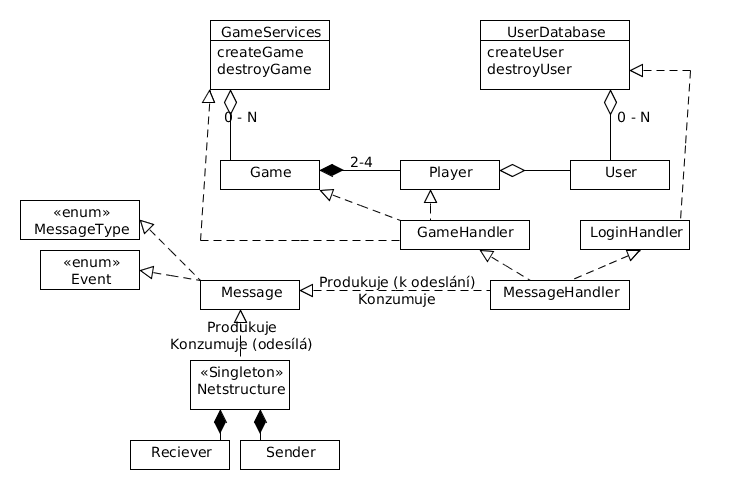
\includegraphics[bb= 0 0 730 490 , width=12cm]{server.png}
\caption{Diagram vztahů tříd v implementaci serveru aplikace.}
\label{fig:game}
\end{figure}

Záznamy o přihlášených uživatelích jsou spravovány třídou \texttt{UserDatabase}. Po přihlášení je vytvořen záznam o uživateli (instance třídy \texttt{User}) Obdobně jako u uživatelů záznamy o vytvořených hrách spravuje třída \texttt{GameServices}. Umožňuje vytváření her (instancí třídy \texttt{Game}) a následné přihlašování hráčů. Po přihlášení (pomocí \texttt{GameServices}) do hry je založena obalová struktura \texttt{Player}, která slouží ke korektnímu spravování situací, kdy se odhlásil hráč (neexistuje instance \texttt{User}). Po odstartování hry není možné měnit počet hráčů ve hře.

\subsubsection{Třída Message}
Objekt pro reprezentaci síťové zprávy v aplikaci. Základními parametry jsou uživatelský soket odesílatele (příjemce), dva typy zpráv \texttt{Event} a \texttt{Message Type} a samotný obsah zprávy ve formátu řetězce.

\subsubsection{Třída Sender}
Odpovědností třídy \texttt{Server} je korektní odeslání všech objektů. Dle typů zprávy sestaví řetězec, který následně odešle příslušným soketem ke klientovi.

\subsubsection{Třída Receiver}
Odpovědností třídy \texttt{Receiver} je korektní přijímání zpráv na soketech. Vlákno pravidelně kontroluje stav soketů a v případě nutnosti vytvoří objekt typu zpráva a zařadí ho do fronty ke zpracování. 

\subsection{Třída MessageHandler}
Odpovědností pracujících vláken třídy \texttt{MessageHandler} je zpracovávat požadavky zařazené do fronty ke zpracování. Během zpracování je pomocí kódů vybraná správná obsluha.


\subsection{Klient}

Architektura klienta je obdobná serveru. Existují zde dvě základní vlákna pro komunikaci \texttt{Sender} a \texttt{Reciever} obalené třídou \texttt{NetStructure}, která je aplikačním jedináčkem. V této třídě je umístěna blokující fronta přijatých zpráv ke zpracování. Opět zde herní struktury ovlivňuje třída \texttt{MessageHandler}.

Klient dodržuje základní prvky architektury MVC. Grafické uživatelské rozhraní je pouze obrazem datových struktur, které jsou plněny výsledky síťových operací. Při každé změně datových struktur je vyvolána aktualizace uživatelského rozhraní.


%========================================
%========================================
%========================================
%========================================
%========================================
\section{Uživatelská příručka} %======================================================================================

%========================================
%=====================================================================================================================
\subsection{Překlad, sestavení a spuštění }

Pro vlastní překlad a sestavení programu ze zdrojových kódů jsou připraveny skripty pro automatické nástroje Ant a Make. Předpokládá se přítomnost Javy (programů java a javac) verze 8 s podporou JavaFX (GUI) pro korektní překlad a spuštění klienta. Pro překlad serveru je v makefile použit překladač gcc respektive g++.


\subsubsection{Klient}
Soubor \texttt{build.xml}, který slouží k sestavování a spouštění klienta aplikace je umístěn ve složce \texttt{MilostnýDopisClient}. Obsahuje základní cíle pro sestavení aplikace, vytvoření jar souboru a spuštění. Pro překlad programu je nutná přítomnost knihoven ve složce \texttt{lib}. Konkrétně jde o knihovny Log4J ve verzi 2.3., která je použita pro logování, a JUnit ve verzi 4.12, která zajišťuje zprostředkování jednotkových testů. Výsledek sestavení naleznete ve složce \texttt{out/ant}. Potřebné knihovny jsou ve složce \texttt{lib} připraveny.

Po spuštění aplikace se otevře přihlašovací okno, kde je nutné vyplnit přihlašovací údaje k serveru. Po přihlášení se do již vytvořené lze připojit pomocí dvojkliku na zvolenou hru. Pokud nejsou žádné hry viditelné je třeba je vytvořit a nebo zobrazit již rozehrané.

Po úspěšném přihlášení se otevře okno s hrou kde uživatel vidí celkový stav hry. Červený trojúhelník ukazuje na aktivního hráče. Pokud je třeba vybrat hráče a cíl efektu karty učiníme tak kliknutím na zadaného hráče. Pro nápovědu efektu karty je třeba najet myší na kartu o které chceme zobrazit nápovědu.

Při výpadku spojení mezi klientem a serverem se klient po vypršení časovače jednou pokusí o opětovné připojení. Během opětovného připojení je uzavřeno okno hry. Klient se automaticky pokusí přihlásit posledního známého uživatele. Pokud bude pokus o přihlášení úspěšný, je možné se opět připojit do rozehrané hry. Pokud pokus selže (server odpovídá \uv{neznámý úživatel}) je záznam o předchozím přihlášení odstraněn.

\subsection{Server}

Soubor \texttt{Makefile} pro překlad serveru je umístěn ve složce build vedle složky MilostnyDopisServer, kde jsou umístěny zdrojové kódy aplikace. Výchozím cílem makefile je sestavení serveru, dále lze využít cíle clean a cleaAll pro vymazání souborů potřebných pro sestavení. Hlavním cílem a tedy spustitelným souborem je \texttt{MilostnyDopisServer}.

Server při spuštění reaguje na parametry příkazové řádky, které lze zobrazit pomocí parametru -h. Výchozí spuštění serveru provedete pomocí příkazu \texttt{./MilostnyDopisServer -r}. Takto spuštěný server naslouchá všechna příchozí spojení na portu 2525. Za běhu serveru lze zjišťovat stav serveru napsáním \texttt{users} pro získání seznamu registrovaných uživatelů, \texttt{games} pro získání seznamu existujících her na serveru a \texttt{konec} pro ukončení serveru. Pro korektní ukončení serveru lze použít i kombinaci kláves Ctr+C, respektive signál SIGINT. 

%========================================
%========================================
%========================================
%========================================
%========================================
\newpage
\section{Závěr}  %======================================================================================================
V rámci této jsem vytvořil dva programy pro simulaci karetní hry Milostný dopis. Prvním programem je server, který je napsán v programovacím jazyce C/C++. Server paralelně obsluhuje více her a hráčů a umožňuje opětovné připojení klienta. Druhým programem je grafický klient k vytvořenému serveru, který je zpracován v programovacím jazyce Java.

\end{document}